\chapter{Lexer}
In this chapter the requirements of the lexer for NISSE will be presented, along with a listing of the tokens for NISSE.
\section{Requirements}
Requirements for the lexer:
\begin{itemize}
		\item The lexer should be able to take any plain text file as input.
		\item The lexer should be able to recognize the input and make tokens according to the token list for NISSE.
		\item The lexer should be able to output meaningful error messages when it cannot match the input to any token.
		\item The lexer should be able to output the tokens so that the parser can use them.
\end{itemize}

\newpage
\section{Token List}
In order to create the syntax in chapter \ref{SSyntax}, tokens have to be identified for later use.
\\ \\
The tokens for the language are as follows:

\begin{lstlisting}[frame=single, caption={Token List of NISSE in EBNF.}]
char            = ? [a-�A-�]+ ? ;
digit           = ? [0-9]+ ? ;
underscore = '_' ;
hyphen = '-' ;
dotv1           = '.' ;
commav1         = ',' ;
space           = ' ' | '	';
atsign          = '@' ;
lcurly          = '{' ;
rcurly          = '}' ;
pipe            = '|' ;
fslash          = '/' ;
bslash          = '\' ;
colon           = ':' ;
scolon          = ';' ;
blist           = '*' ;
nlist           = '#' ;
percent         = '%\%%';
exclamation     = '!' ;
eolv1           = \r | \n | \r\n ;
format_kwd      = '@u' | '@b' | '@i' | '@apply' | '@image' | '@title' | '@subtitle' | '@note' ;
setting_kwd     = '@setting' ;
begin_kwd       = '@begin' ;
end_kwd         = '@end' ;
url             = '@url' ;
\end{lstlisting}

\noindent{The abnormal in this token list is \texttt{``format{\_}kwd''}, \texttt{``setting{\_}kwd''}, \texttt{``begind{\_}kwd''} and \texttt{``end{\_}kwd''}, (kwd is short for: keyword). These keywords are explicit, because in the productions in which they occur they can only be on the left hand side of a left curly bracket. Their specific use is explained in chapter \ref{SSyntax}.}
\\ \\
The reason each special keyword has its own token and not a general production, is to easily see the difference between the special tokens and the normal ones, without the need to check that a given token in the syntax analyser is the right token.
\\ \\
\texttt{``Char''} is used whenever characters needs to be used in the code. Char is used both for plain text and identifiers. \\
\texttt{``Digit''} is used whenever numbers need to be used in the code. \\
When numbers or characters are expected, then one such has to occur at least once.

\subsection{NFA}
Figure \ref{fig:nfaer} is a NFA (Nondeterministic Finite Automaton) for when the user inserts an \texttt{at sign}, which can become a lot of different tokens. It will always take an input before an epsilon\footnote{the empty set}, for instance, if an \texttt{at sign} and an \texttt{i} is written, it looks at the next tokens, before it uses the epsilon transition.

\begin{figure}[h!]
	\centering
		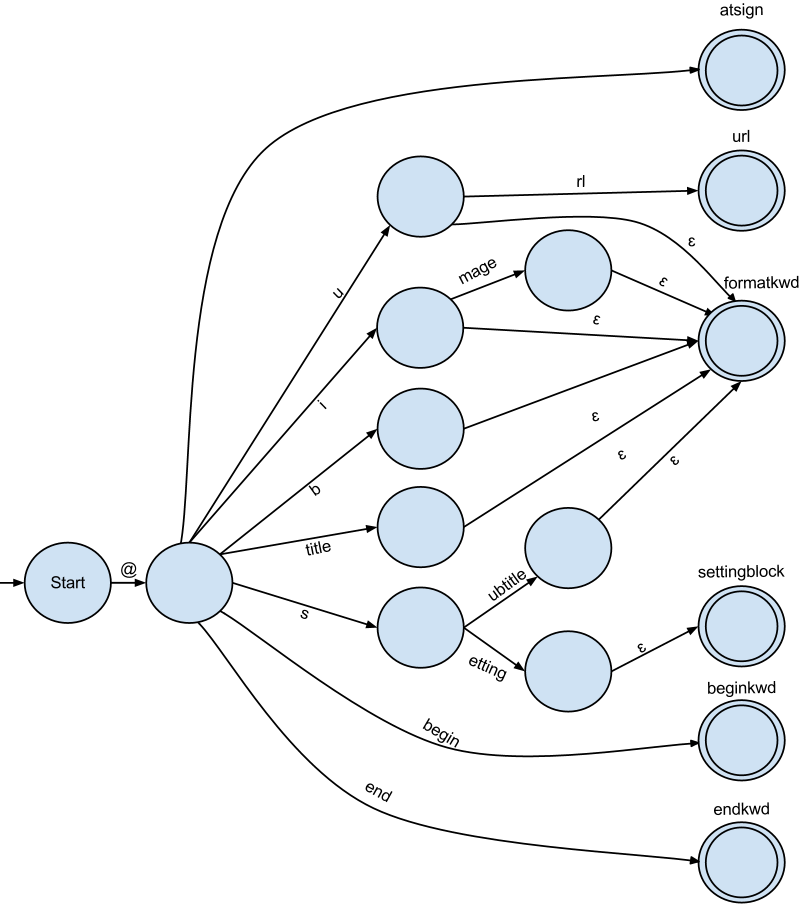
\includegraphics[width=0.9\textwidth]{./images/nfaer.png}
	\caption{NFA for atsign}
	\label{fig:nfaer}
\end{figure}

The \texttt{at sign} can create a number of different tokens, shown in figure \ref{fig:nfaer}, these are \texttt{Formatkwd, settingblock, beginkwd, endkwd, url} and if the text does not match any of that, it is tokenized as an \texttt{at sign} and the text after the \texttt{at sign} is tokenized as a \texttt{character}.

\subsubsection*{Regular expression}
The regular expression for figure \ref{fig:nfaer} is shown in listing \ref{lst:Regularexpression}
\begin{lstlisting}[frame=single, caption=Regular expression, label=lst:Regularexpression]
%$@ ( (i (\epsilon \cup mage)) \cup (u ( \epsilon \cup rl)) \cup b \cup title \cup (s(ubtitle \cup etting)) \cup begin \cup end \cup \epsilon)$%
\end{lstlisting}